\documentclass[como,a4paper,12pt,final]{Classes/c4e-preprint}
\graphicspath{{Figures/}}

%--------------------------------------------------------------------
%    LaTeX includes
%--------------------------------------------------------------------
% Note subfig is now deprecated.
\usepackage{subfig}
\usepackage{graphicx}
\usepackage{xspace}
\usepackage{multirow} % added by klb83

%--------------------------------------------------------------------
%    pdf properties (must be consistent with title page data below)
%--------------------------------------------------------------------
\hypersetup{
  pdftitle={Structure and properties of curved polycyclic aromatic hydrocarbon nanoclusters},
  pdfauthor={Kimberly Bowal\affiliated{1}, Jacob W. Martin\affiliated{1,2}, Markus Kraft\affiliated{1,2,3}}
  pdfsubject={c4e preprint template},
  pdfkeywords={c4e, preprint, template}
  }

\begin{document}
%--------------------------------------------------------------------
%    title page (must be consistent with pdf properties above)
%--------------------------------------------------------------------
\title{Self-assembly of curved aromatic molecules in nanoparticles}
% Investigating the self-assembly and structure of nanoparticles containing curved carbons
\author{Kimberly Bowal\affiliated{1}, Jacob W. Martin\affiliated{1,2}, Markus Kraft\affiliated{1,2,3}}
\keywords{curved polycyclic aromatic hydrocarbon, nanoparticle, self-assembly, internal structure, mesophase}
\nopreprint{XXX} \nopreyear{2020} \releasedate{XXX}

\affiliation{1}{
  Department of Chemical Engineering \\and Biotechnology\\
  University of Cambridge\\
  West Site, Philippa Fawcett Drive\\
  Cambridge, CB3 0AS\\
  United Kingdom\\
E-mail: \href{mailto:mk306@cam.ac.uk}{mk306@cam.ac.uk}}
  
\affiliation{2}{
  Cambridge Centre for Advanced Research\\
  and Education in Singapore (CARES)\\
  CREATE Tower, 1 Create Way\\
  Singapore, 138602}

\affiliation{3}{
  School of Chemical and\\ Biomedical Engineering\\
  Nanyang Technological University\\
  62 Nanyang Drive\\
  Singapore, 637459}



\maketitle

%--------------------------------------------------------------------
%     abstract
%--------------------------------------------------------------------
\begin{abstract}
The internal and surface structure of nanoparticles containing curved polycyclic aromatic hydrocarbons (cPAHs) are investigated using molecular modelling. Due to the inclusion of one or more five-membered rings within their hexagonal lattice, these polar fullerene-like molecules possess unique steric and electronic properties that make them good candidates for many applications including microporous materials for gas storage, organic electronic devices such as imaging probes and batteries, sensors, and micelles for targeted nanomedicine. Development of these applications requires an understanding of the self-assembly and nanostructure of cPAH nanoparticles, which has not yet been well explored. This work uses replica exchange molecular dynamics to determine the energy-dependent nanostructure of cPAH particles. The interactions between cPAH molecules are described using the new curPAHIP potential. A range of cPAH sizes and ratios are investigated, along with systems containing planar PAHs and ions, to explore the homogeneous and heterogeneous particle internal arrangements and properties. Homogeneous cPAH particles are found to be tightly packed and less stacked than their planar PAH counterparts. The constituent cPAH size plays a role in the molecular arrangement, with large 15 ringed cPAHs (\ce{C42H14}) displaying stacked configurations absent in nanoparticles containing small 7 ring cPAHs (\ce{C20H10}). Heterogeneous particles containing cPAHs of different sizes display a core-shell structure in which the larger molecules make up the core and the smaller molecules comprise the shell, as seen with planar PAH nanoparticles. %This trend is not strongly influenced by the molecule ratio. 
In addition, the presence of planar PAHs and ions within cPAH nanoparticles promotes distinct arrangements dominated by weak dispersive interactions and strong electrostatic interactions, respectively. These systems may be indicative of nanoclusters generated in processes such as combustion. These results provide new information on structures and properties of nanoparticles containing cPAHs, including density, molecular structure, and surface composition. This provides valuable understanding of the self-assembly and structure of nanoparticles with great potential in many applications.

%Curved carbon materials arise from the inclusion of non-hexagonal rings within a hexagonal lattice and exhibit unique steric and electronic properties. These fullerene-like molecules are candidates for many applications including gas storage, batteries, imaging probes, and targeted nanomedicine. Development of these technologies requires an understanding of the self-assembly and dynamic nanostructure of particles containing curved carbons, which has not yet been well explored.
%This work uses advanced molecular dynamics simulations to explore the properties of nanoparticles containing curved carbons. Intermolecular interactions were described using the recently developed curPAHIP potential able to capture the enhanced interactions caused by the flexoelectric effect. Large timescales and temperature ranges were sampled to provide insight into the dynamic behaviour of curved aromatics in homogeneous systems as well as those containing planar molecules and cations. The size and ratio of constituent fullerene-like molecules have significant effects on the internal structure and surface properties of nanoparticles. These results provide information on the energetic and structural properties of cPAH-containing nanoparticles, useful for an accurate understanding of the dynamic nature of these systems.

%Understanding the formation and properties of soot particles is critical for the accurate description of turbulent reacting flows within combustion. Due to the small time and length scale of these particle dynamics, a complete description of soot particle properties has remained a challenge. Curved polycyclic aromatic hydrocarbons (cPAHs) have been identified as key constituents of soot particles and we have recently shown that their interactions with ions may contribute significantly to particle formation (Bowal, K, et al. "Ion-induced soot nucleation using a new potential for curved aromatics'', Combustion Science and Technology (2018, accepted)). The structural properties of cPAH clusters are unknown and further molecular modelling studies are required to provide insight into the clustering behaviour of cPAHs - their size-dependent arrangements, interactions with planar PAHs, and assembly around ions.

\end{abstract}

%%\begin{figure}[!ht]
%%    \setlength{\figwidth}{12cm}
%%    \centering
%%    \resizebox*{\figwidth}{!}{\includegraphics{GraphicalAbstract.pdf}}
%%\end{figure}

\textbf{Highlights:}

Self-assembly of binary systems of curved aromatics
\begin{itemize}
\item Can we describe the intermolecular interactions of cPAH? (curPAHIP, isoPAHAP, DFT and SAPT(DFT)).
\item How do cPAH self-assemble into a mesophase? (homogeneous - alignment angles compare with x-tal DFT, coordination number and intermolecular spacing - stacking, carbonisation mixtures)
\item Do cPAH self-assemble into core-shell nanoparticle? (heterogeneous - radial distance, planar and curved phase separate Janus particles)
\item How do cPAH self-assemble around ions (energies, structural differences).
\end{itemize}

\vfill

%--------------------------------------------------------------------
%     table of contents
%--------------------------------------------------------------------
\clearpage \setcounter{tocdepth}{3} \tableofcontents

%--------------------------------------------------------------------
%     paper body
%--------------------------------------------------------------------
\clearpage
%use input{} to include the body of the preprint
\newcommand{\curPAHAP}{curPAHIP\xspace} 
%
\section{Introduction}
\label{sec:Introduction}
% Answering: What is the energy/structure of cPAH particles? How does this differ from fPAH particles? What is the influence of molecule size, proportion, and presence of ions or fPAHs?

%% Curved carbons are everywhere...
Curved carbons are found in many materials including porous carbons (ref), glassy carbons (ref), and soot particles (ref).
% curvature (ie defects) integrated easily in (production) processes
% Mesophase pitch is used to produce many materials, including synthetic graphite.

HRTEM analysis of coals show that a significant proportion (28-49\%) of the constituent molecules are curved (with a structure corresponding to centrally located pentagonal rings in aromatic structures) (10.1021/acs.energyfuels.5b02907, 10.1016/j.carbon.2017.02.059). This results in a low degree of order and poor stacking (only ~20\% stacked) (10.1016/j.carbon.2017.12.106).


%% Curvature is caused by... (incl experimental refs)
This curvature is caused by the presence of non-hexagonal rings, such as pentagons, within a hexagonal lattice. The resulting molecules have steric and electronic properties not present in carbon materials containing hexagonal structures only (without defects). In particular, curved carbon-based molecules possess a dipole moment due to the flexoelectric effect (ref). This allows curved molecules to interact in long-range electronic (dipole-dipole) interactions not present in systems containing planar carbon molecules.
% even important in small proportions since seem to interrupt formation of mesophase...
The presence of curved aromatic molecules influences material structure and properties. For example, the integration of curvature in molecules is crucial in determining whether a combusted wood-based material produces graphitic or non-graphitised carbon \cite{abrahamson2018carbon}. This suggests that curved aromatic molecules prevent graphitisation by disrupting formation of the mesophase. %diminishes anisotropy which provides reduced connectivity in lower (1 and 2) dimensions.

%% Arrangement of atoms determines everything...
The arrangement of atoms in a carbon material determines its structure, properties, and function. Nanostructure is crucial to understand the existing and potential behaviour of carbon materials. For example, to understand (how to optimise) a structure's stability/longevity, environmental interactions, and ability to store other molecules - all vital for gas storage, drug delivery, or sequestration applications.  Similar information about the detailed structure of the material is required for other applications such as batteries, adsorbents, %involving thermal protection, conductivity.
sensors, and novel nanocarbon materials.
In addition to providing the understanding required to optimise the nanostructures for these applications, this provides insight into the natural processes and environments that generate nanoparticles containing polycyclic aromatic hydrocarbons, such as combustion-produced pollutants (ref) and interstellar medium (ref).

Add in: the presence of curved carbons is shown to increase the nanostructure porosity, providing enhanced adsorption important for applications such as carbon sequestration (10.1021/acs.energyfuels.9b04418).

Also add in: carbon materials have been fabricated for use as adsorbents, carriers, catalyst supports, electrodes, and other advanced applications (refs).  The performance of these materials can be directly improved/tuned for these applications by adjusting their physical properties - in particular their nanostructures.  It is therefore crucial to develop a detailed understanding of the molecular interactions involved to enhance the prediction and design of desired carbon nanostructures.


%% curved carbon applications...
%Curved carbons have great promise in many applications such as understanding particulates, novel nanocarbon materials, sensors
%Microporous materials: gas storage, separation
%Organic electronic devices: imaging probes, batteries
%Nanomedicine: sensors, targeted micelles
%Nanoparticle formation: soot, carbon blacks, atmosphere
%Applications: Lithium ion batteries, electronics, fuel cells


%% Previous work looking at cPAH interactions:	Homogeneous dimers
Previous work on polycyclic aromatic hydrocarbons (PAHs) has focused on flat/planar PAHs (fPAHs), with less attention given to curved PAHs (cPAHs). However, electronic structure calculations show that there is significant energy in interactions between nested concave-to-convex homogeneous cPAH dimers, showing that curvature does not prevent dimers from forming pi-pi stacked assemblies similar to planar systems (10.1002/qua.21794, 10.1002/jcc.25084). As with fPAHs, cPAH dimer interactions are dominated by $\pi$-$\pi$ interactions compared to CH-$\pi$ interactions. However cPAHs in the concave-convex dimer configuration show different behaviour than fPAH dimers and cPAHs in convex-convex configuration, with the eclipsed dimer (in which the aromatic planes are aligned) showing a higher stability than the staggered dimer (in which the aromatic planes are shifted relative to each other) (10.1016/j.cplett.2011.07.030, 10.1002/jcc.25084).
Dispersion provides the dominant energy contribution, although electrostatics are also significant especially in contrast to fPAH dimers (10.1002/jcc.25084, 10.1016/j.cplett.2011.07.030). 
%Pi-pi > pi-CH interactions, eclipsed > staggered.

Different degrees of curvature can result in increased or decreased cPAH dimer strengths, due to geometry and (less so) electrostatic effects. Curvature is able to increase interaction strength by decreasing C-C distances for increased dispersion interactions (10.1021/jp305700k). 
However, very curved PAHs have lower interaction strengths similar to fPAHs due to increased steric hinderance (10.1016/j.proci.2018.05.046, 10.1002/qua.21794). High curvature also increases exchange-repulsion and can destabilise the dimer (10.1021/jp305700k, 10.1002/qua.21794).


%% Previous work looking at cPAH interactions:	Bulk systems
Analysis of the crystal structure of cPAHs shows a molecule size dependent behaviour. Corannulene (\ce{C20H10}) is the smallest cPAH, containing one central pentagon with five surrounding hexagonal rings (shown in Figure XXX). Corannulene has no long-range stacked order in crystal analysis (10.1107/S0567740876012430, 10.1021/jo050233e, 10.1021/acs.analchem.8b05260, 10.1016/j.carbon.2015.06.041, 10.1021/ar950197d). 
%CH-pi interactions dominate. Shallow bowl, rapid bowl inversion.
CH-$\pi$ interactions, in which the posivitely charged rim of one molecule is almost perpendicular to the negative region and the bottom of the other molecule in a T-shaped configuration, exists in the corannulene crystal (10.1515/znb-2010-0403). This is supported by evaluation of the electrostatic potential of corannulene.

In contrast, cPAHs with increased size, curvature, rigidity, and/or heteroatoms form columnar stacks (10.1021/ar950197d, 10.1039/C39940002571, 10.1021/ja0123148, 10.1021/ja970845j, 10.1021/acs.jpcc.6b10895, 10.1016/j.carbon.2015.06.041, 10.1002/anie.200460855, 10.1021/om040131z, 10.1021/cg100898g, 10.1021/ja0518169, 10.1039/A905860E, 10.1515/znb-2010-0403, 10.1021/cr050554q). These systems show larger $\pi$-$\pi$ overlap and staggered stacked interactions to produce extended $\pi$ networks enhanced by CH-$\pi$ interactions.


%% Limitations of existing work
To date, detailed studies of cPAHs have primarily included static DFT calculations or crystal structure experiments, as described above, neither of which provide information about intermolecular dynamics and particle nanostructure.


%% Previous work looking at cPAH interactions:	Heterogeneous systems (dimers, etc)
% need to do a better job at splitting ideas: increased electrostatics and interactions with ions vs different structure and bowl complementarity
Computational studies of fPAHs show that, unlike cPAHs, heterogeneous dimers are significantly weaker than their homogeneous counterparts (ref). This heterogeneity was shown to decrease the stability of a nanoparticle containing different molecule sizes and lead to a distinct partitioning in which the larger molecules formed the cluster core and the smaller molecules resided in the outer shell \cite{bowal2018partitioning}. Dynamic interactions of cPAHs or fPAHs with cations also highlighted the ability of cPAHs to engage in electrostatic interactions that stabilise a cPAH cluster, while fPAHs cannot \cite{bowal2019ion}. These results suggests that the fundamental interaction differences between fPAHs and cPAHs may cause different clustering and packing behaviours. Preliminary work suggests that the nanostructure of homogeneous cPAH clusters is significantly different from similar-sized fPAH clusters \cite{bowal2019ion}, and perhaps different molecule sizes will show increased packing and stability due to bowl complementarity.
% This may be more representative of the experimentally observed structure of nascent soot particles.

%So expect homogeneous corannulene nanocluster to be disordered, homo 2pent15ring cluster to have stacks. Expect mixed cPAH cluster to be dominated by 2pent15rings but enhanced corannulene stacking and more stable than comparable mixed fPAH cluster.
% cPAH interactions with different sized molecules (no heteroatoms) (refs????). Increased stability compared to heterogeneous fPAH systems because of shape fitting and enhanced electrostatics and CH-pi interactions (?).
%Homodimers are weaker than heterodimers because they don't take advantage of bowl complementarity (10.1002/jcc.25084).
%Thus we hypothesise that heterogeneous cPAH clusters may be more stable than their heterogeneous fPAH counterparts since different sizes of cPAHs may provide stable packing arrangements.

%% Previous work looking at heterogeneous fPAHs…
%Previous work examined heterogeneous PAH clusters using replica exchange molecular dynamics \cite{bowal2018partitioning}...
% Explain how this work is extending previous work done on fPAHs (internal structure/partitioning, surface properties) - or should this essentially go in the methods section?

%% purpose of this work... 
The structural properties of cPAH clusters are unknown and further molecular modelling studies are required to provide insight into the clustering behaviour of cPAHs - their size-dependent arrangements in both homogeneous and heterogeneous systems, interactions with planar PAHs, and assembly around ions. Understanding non-covalent interactions with and between curved carbon nanostructures has importance in many systems and great potential for numerous applications.
% Development requires understanding of self-assembly and dynamic nanostructure of curved aromatics

The purpose of this work is to explore properties %(molecular arrangements, melting points, densities, surface properties, etc) 
of clusters containing curved PAHs, with the aim of answering the following questions: Are cPAH clusters more stable than fPAH clusters? Do cPAHs partition within clusters the same way fPAHs do? What is the internal nanostructure and surface composition of cPAH particles?  
%Predict long-range dipole-dipole interactions increase stability.
In this work, we are motivated to understand the influence of cPAHs in soot particle structure and stability, but these results have general relevance to nanoparticles containing cPAHs regardless of source or application.
%Hypothesis: cPAH clusters are more representative of the experimentally observed structure of nascent soot particles, heterogeneous cPAH clusters are significant since they are stable than their fPAH counterparts.
This is important for better understanding of soot particle formation and growth, and has implications for other carbon nanomaterials such as batteries, imaging probes, gas storage, optoelectronics, and targeted nanomedicine.
We will address these questions in this work by studying nanoparticle systems containing cPAHs, first in homogeneous clusters containing one molecule type only, then extending this to heterogeneous clusters to understand the interactions and effect of cPAH size and ratio. Finally, exploratory work on systems containing cation(s) and fPAHs is presented.


%%%%%%%%%%%%%% Other notes to perhaps include %%%%%%%%%%%%%
%Pi-pi interactions play a pivotal role in so many super important processes (the way proteins fold and drugs bind to targets, crystal packing and charge transport properties in organic electronics, materials) - see references “Pi-pi Stacking of Curved Carbon Networks: The Corannulene Dimer” in Mendeley

%Relevance to carbon (quantum) dots?




\section{Methods}
%% systems 
Clusters studied: homogeneous (corannulene, 2pent15ring each: 25, 40, 50, 100, [200]), heterogeneous (20/20, 10/30, 30/10).
40 corannulene with 1 K+ and 2 K+.
We should note that in this work, the terms (nano)particle and cluster are effectively synonymous: a nanoparticle is a cluster of molecules.

%% curPAHIP
%Reintroduce curPAHIP potential
We have previously developed an atomic potential for cPAHs, based on the intermolecular potential for planar PAHs 

As with the corannulene molecules (reported in detial in CST paper), the 2pent15ring molecule is minimised. Mass-less atoms are added at a distance of 0.52 \AA above each of the pentagonal carbon atoms to provide a dipole moment of 5.2784 D (within <1 \% of dipole calculated using DFT). The atomic coordinates and charges of the minimised 2pent15ring monomer are provided in the Supplementary Information.


%%%%% Computational details %%%%%
Replica exchange molecular dynamics, position potential (Gromacs 5.1.4, mixed initial configurations using packmol, 3 ns, 60-75 replicas, 200 - 1600 K).


%%Density functional theory.
%Monomers and minimum energy dimers calculated using geometry optimisation at B97D/6-311G(d,p) with frequency calculation to ensure suitable minima was found.  Single point calculation, with BSSE correction, at B97D/cc-pVTZ for all dimers.
Density functional theory (DFT) calculations are used to determine the structure of cPAH monomers and configurations and energies of cPAH dimers. The B97-D functional \cite{grimme2006semiempirical}, a hybrid functional with an empirical dispersion correction, is used in this work.  Geometry optimisations are carried at the B97-D/6-311G(d,p) level of theory with frequency calculations to ensure suitable minima are found, and subsequent single point calculations use B97-D/cc-pVTZ, with basis set superposition error corrections.  These functional and basis sets were selected since they provide good agreement (within 4\%) with benchmark CCSD(T) \cite{janowski2011convex} and SAPT(DFT) \cite{Cabaleiro-Lago2018} calculations of corannulene dimers. %and have been used in previous studies looking at cPAHs (Preprint 207)


%%%%% Analyses %%%%%
%Melting point analysis.
The REMD method allows rapid evaluation of equilibrated systems, but the replica swapping process hides local ensemble information such as a change in energy due to melting. This means that information about the cluster melting points could not be extracted from the REMD simulations. To assess the melting points of these systems, individual 1 ns simulations using classical MD were conducted at each desired temperature from the final REMD configuration. No position potentials were implemented for these post-REMD MD simulations.
%Melting points are identified using both energy- and movement-based metrics, as in previous works (many refs).
%Previous experimental and simulation-based studies have shown that a LI value of 0.10-0.15 provides an indication of solid-to-liquid transition temperature (10.1063/1.1426419).

The final 500 ps of the post-REMD MD simulation was used as the production period and is used for analysis.
(The final 500 ps of the post-REMD MD simulations are equilibrated and show <5\% drift in energy so this was selected as the production period.)

% Structural analysis - Molecular arrangement analysis (radial distances, coordination numbers, stacking angle, etc).
A number of different metrics are used to evaluate cluster structural properties. For all metrics, the final 500 ps of the post-REMD simulation (t=3500-4000 ps of total simulation time) with a timestep of 1 ps is used for analysis. Unless stated otherwise, molecular properties consider molecule centres of mass.
These metrics were assessed and represent the corannulene crystal structure well (see the Supplementary Information for more details).


% coordination numbers
A quantitative measure of the degree of stacking order in the molecular structure is provided through the use of coordination numbers. These are calculated as the number of near neighbours within a cut-off radius $R$ of each molecule, averaged over each molecule type. 
%The values of $R$ were selected to include sandwich-type stacked interactions between molecules but exclude molecules more than one layer away. (This means that the equilibrium dimer distances served as the minimum $R$ values for each molecule type). For corannulene molecules this cut-off distance, $R_{\text{ANN}}$, is 0.4 nm, and for 2pent15ring molecules $R_{\text{two}}$ is 0.5 nm.  
% maybe change to say: The values of $R$ are selected based on corannulene unit cell / to
The values of $R$ were selected as the minimum value required for almost all ($\ge 95\%$) of the molecules to have at least one identified neighbour (considering increments of 0.1 nm).  For cluster systems containing corannulene only, this his cut-off distance, $R_{\text{ANN}}$, is 0.7 nm, for clusters containing 2pent15ring molecules only $R_{\text{two}}$ is 0.5 nm, and for clusters containing molecules of both types... % if the heterogeneous systems need different R values.
%Molecules are considered neighbouring if their centres of mass are within the cut-off distance for at least half of the 500 ps analysed simulation.
The sensitivity of these cut-off values on calculated cluster properties is discussed in the Supplementary Information.

 
The mathematical description of the coordination number is provided in the Supplementary Information.
The sensitivity of the coordination number values on these selected $R$ is discussed further in the Supplementary Information.


% alignment angles
Molecular alignment angles are calculated to provide information on the configurations of interacting molecules within the clusters studied.  An alignment angle is defined as the angle between normal vectors to the central rings of the neighbouring cPAHs considered (for corannulene molecules this is the pentagonal ring and for 2pent15ring molecules this is the central hexagonal ring).  Figure XXX provides a schematic of the alignment angle between two neighbouring corannulene molecules.
%As in previous metrics the cut-off distances, $R$, are used to determine neighbouring molecules.  
%
\begin{figure}[!tbh]
\centering
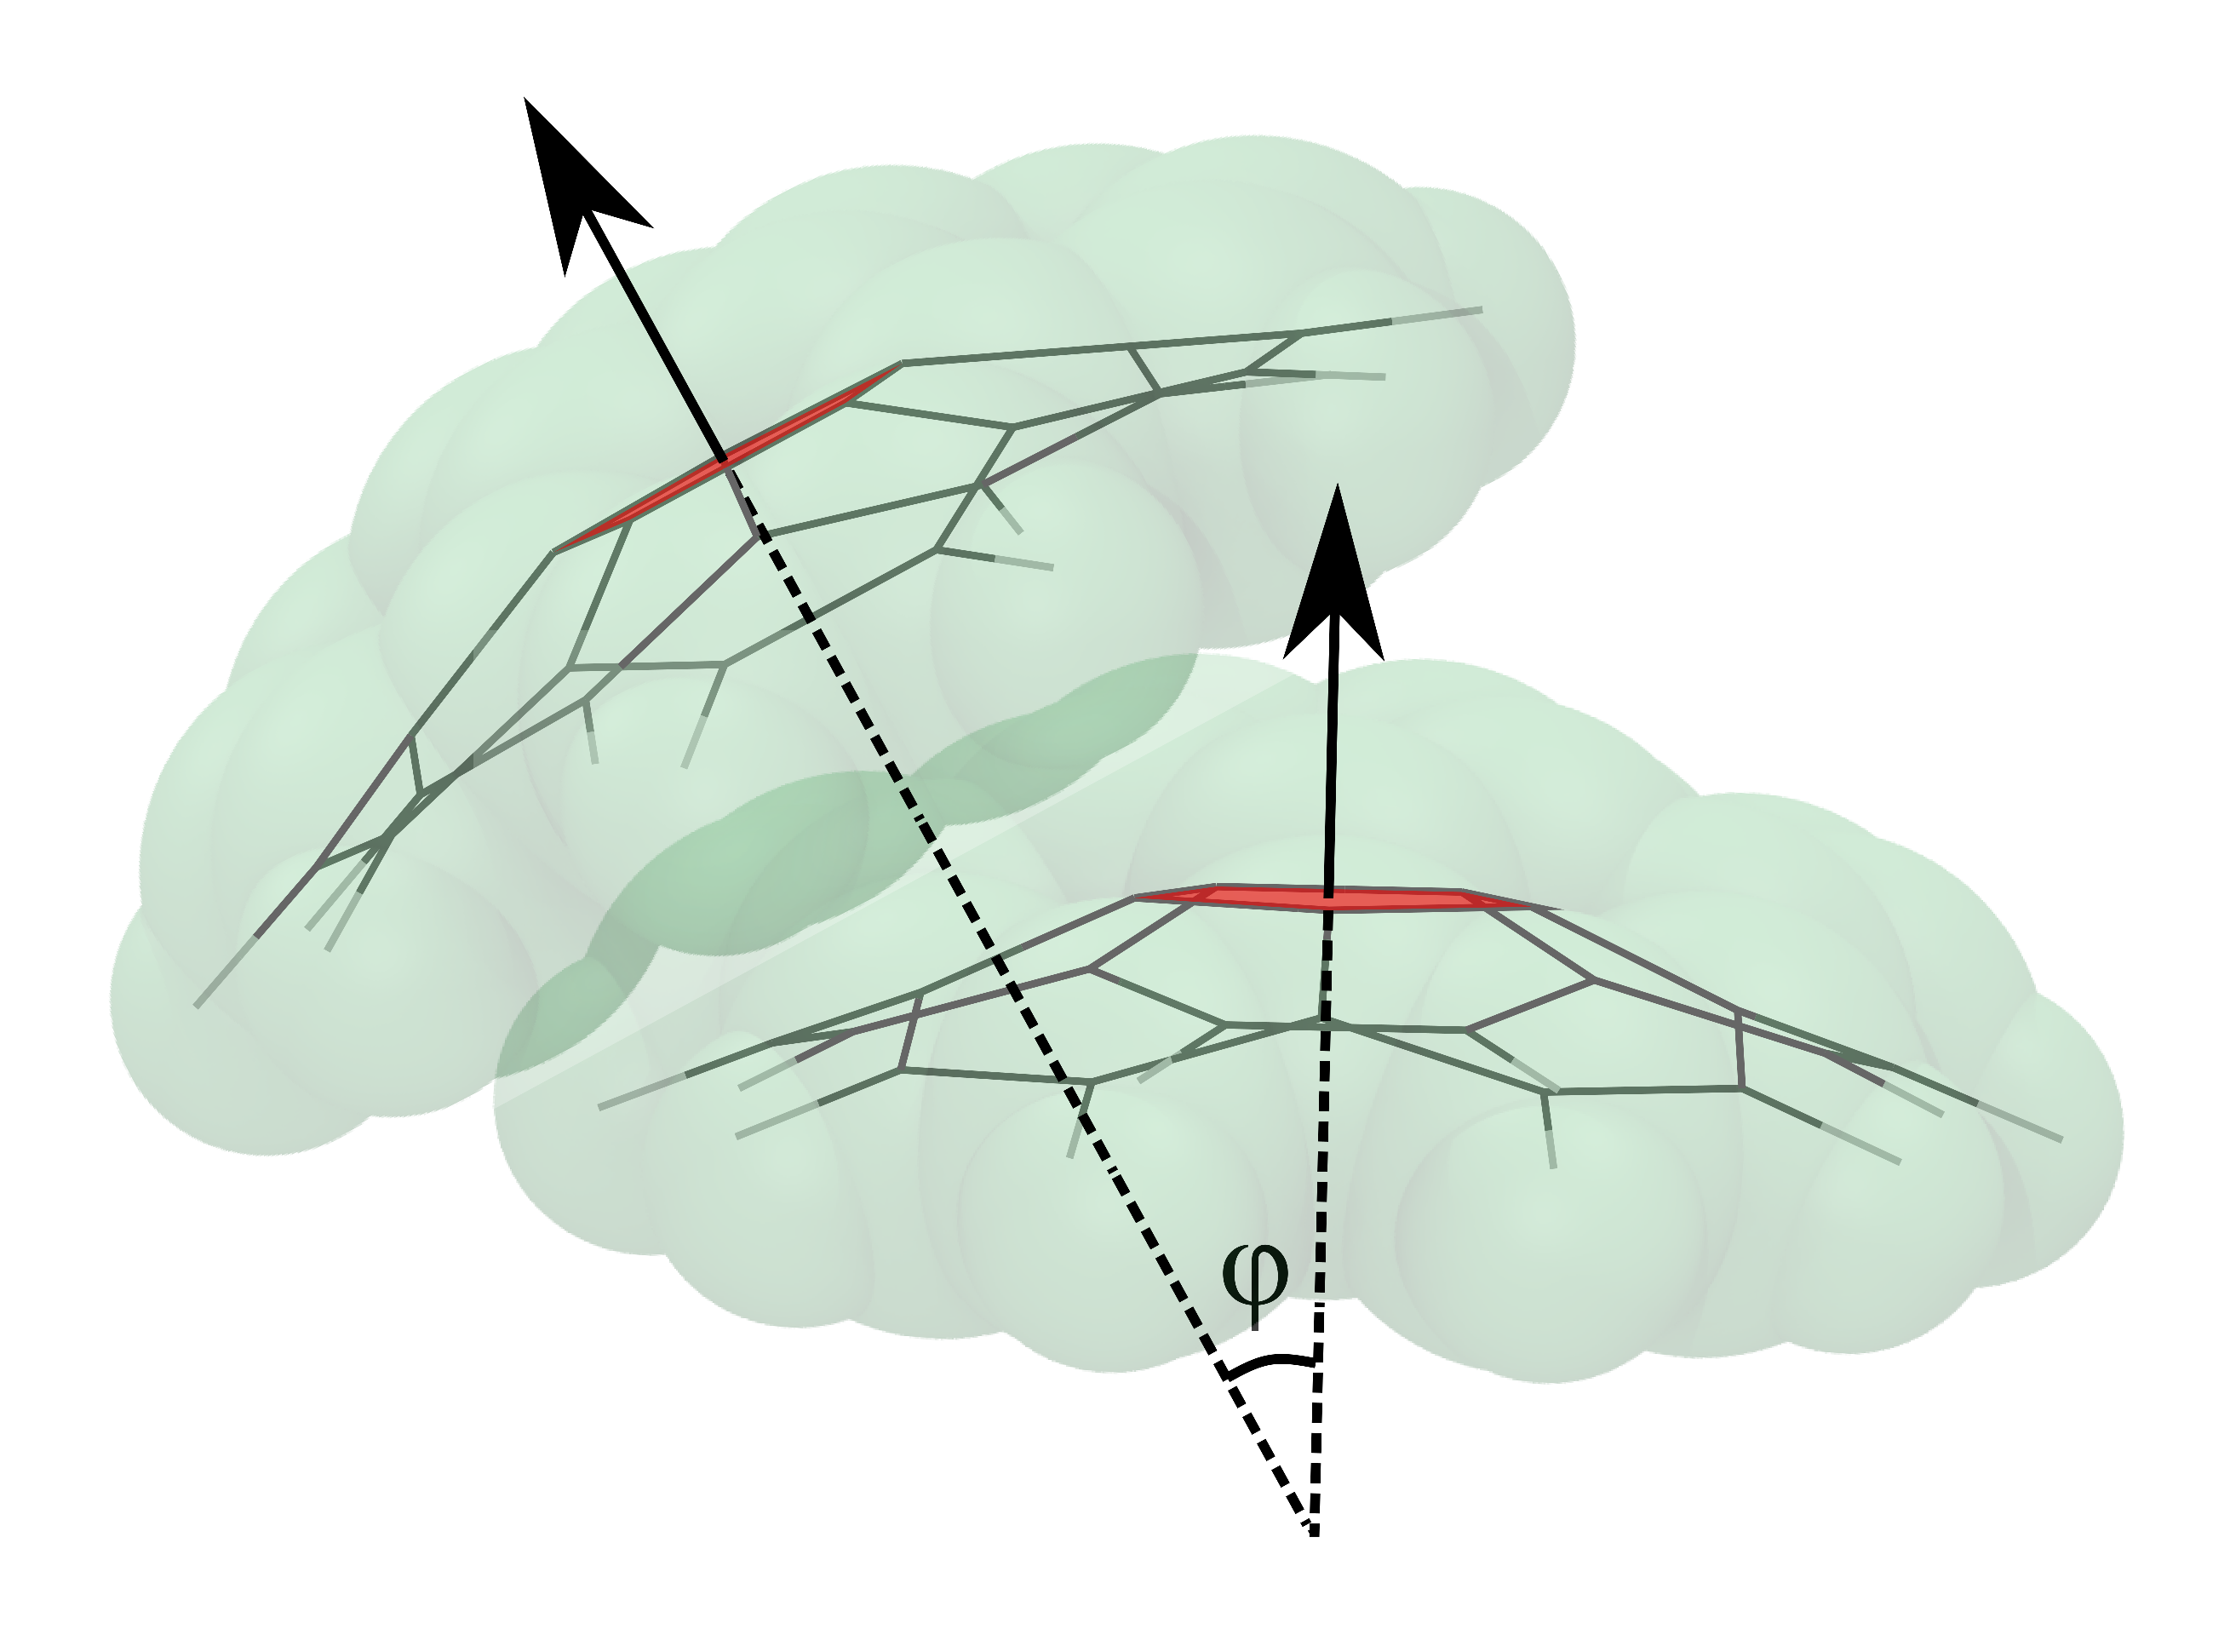
\includegraphics[width=0.25\linewidth]{Figures/alignment_angle_schematic.eps}
\caption{Schematic illustrating the calculation of the alignment angle between two neighbouring corannulene molecules. The central pentagonal rings are highlighted in red and the alignment angle ($\varphi$) is $30^{\circ}$.}
\label{fig:alignmentangle_schematic}
\end{figure}
 

% intermolecular distances - probably don't need to include since covered by more general stuff above!
Intermolecular distances are calculated between each molecule and its neighbours within $R$ and averaged over all equilibrated timesteps (500-1000ps of post-REMD MD simulation, considering each 1 ps).  The reported values are averaged over molecule type interactions in the system, including: all, 2pent15ring-2pent15ring, corannulene-corannulene, and 2pent15ring-corannulene.

% radial distances
Molecular radial distances are defined as the average distance between a molecule type and the cluster centre and provide insight into the molecule type partitioning within the cluster.
% do I need to include an equation (in the SI)?

% surface properties
Surface properties are calculated as the solvent excluded surface area using MSMS X.X (ref). More details about rolling ball algorithm etc...
Configurations from every 50 ps from the production period (from 500-1000ps) are used in this calculation.


\section{Results}
\subsection{Dimer energy assessment} % curPAHIP potential for larger cPAHs - dimer energies
The binding energies of cPAH dimers calculated by DFT calculations are compared to the curPAHIP intermolecular potential to assess the suitability of the latter in describing systems containing cPAHs.  This is shown for four dimer types in Figure \ref{fig:potentialDFTcurves}.  The energy of the isoPAHAP potential is also included to highlight the behaviour of a potential that does not consider molecule curvature.
The curPAHIP potential agrees very well with the DFT and SAPT(DFT) results for the corannulene dimer, Figure \ref{fig:potentialDFTcurves}(a). This is expected, since these \textit{ab initio} values were used in the parameterisation of the curPAHIP potential \cite{bowal2019ion}. 
Figure \ref{fig:potentialDFTcurves}(b) shows that the curPAHIP potential can be extended to cPAH molecules larger than corannulene, since there is good agreement with DFT energies for the larger 2pent15ring molecule (within 5\% of the dispersion-corrected DFT). In contrast, the isoPAHAP gives a minimum energy value that is 31\% smaller than B97D.
Energies of heterogeneous dimers, containing one corannulene molecule and one 2pent15ring molecule, are also well captured by the curPAHIP potential, as seen in Figure \ref{fig:potentialDFTcurves}(c) and (d).  Of note, the nested dimer with the smaller corannulene molecule on the concave side of the larger 2pent15ring molecule (Figure \ref{fig:potentialDFTcurves}(c)) shows a T-shaped type configuration. In this system the curPAHIP potential provides a slightly smaller %need to quantify? 
angle between the two molecules in the minimum energy configuration than the DFT calculation, suggesting that CH-$\pi$ interactions are weaker and $\pi$-$\pi$ overlap is favoured using the intermolecular potential.  This difference does not cause a significant difference in larger systems, however, as discussed further in the alignment angle analysis. % discuss how the dimer angle is seen in the stacks (20 degrees)
In all cases, the isoPAHAP potential significantly underestimates the binding energy and overestimates the equilibrium dimer distance since it does not include the enhanced electrostatics and dispersion due to the flexoelectric effect.
% Overall some slight differences compared to DFT results show repulsive component of curPAHIP is shifted to smaller distances (means that there might be stronger attractions at small dimer separation distances) and minimum is slightly lower energy (provides conservative case if any different (less likely to bond))
% The difference between the DFT and curPAHIP energies can be partly explained by the fact that the MD minimised monomers (used in curPAHIP assessment) are more curved than the DFT monomers. So perhaps the energies are not as low for the curPAHIP potential since the dimers are not able to reach the same small distance values without steric hindrance and repulsion coming into effect.
%
\begin{figure}[!tbh]
\centering
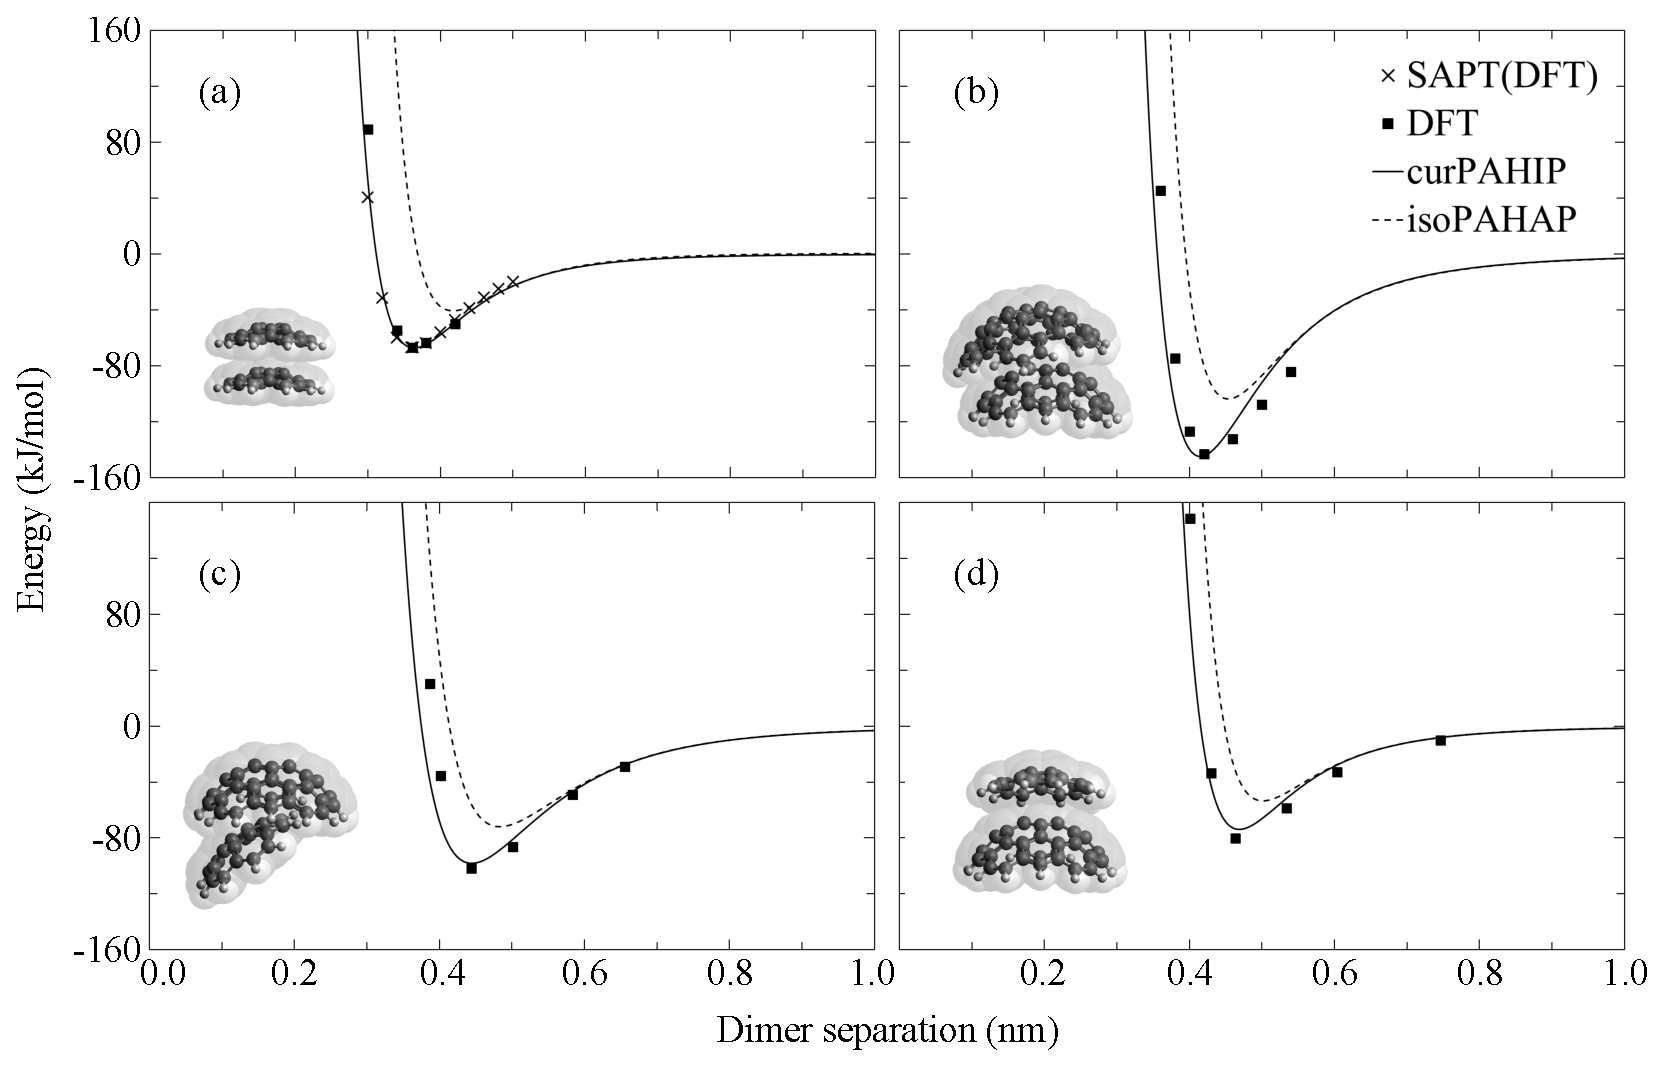
\includegraphics[width=1\linewidth]{Figures/potentialDFT_curves.eps}
\caption{Interaction energy versus separation distance for a cPAH dimers determined from SAPT(DFT) calculations \cite{Cabaleiro-Lago2018}, DFT calculations, the curPAHIP potential, and the isoPAHAP potential. The dimers are as follows: (a) two corannulene molecles, (b) two 2pent15ring molecules, (c) and (d) one corannulene and one 2pent15ring molecule each.}
\label{fig:potentialDFTcurves}
\end{figure}
%
\subsection{Energies}
The intermolecular energies as a function of cluster mass are shown in Figure XXX (tabulated values are provided in the Supplementary Information).  The energies are shown per atom in the system, in order to facilitate direct comparison between systems of different molecule sizes.
It is clearly seen that in all cases the energy decreases with cluster mass, for clusters containing curved or planar PAHs.  Homogeneous clusters containing planar PAHs show relatively consistent energy trends across molecule sizes from pyrene to circumcoronene (all coloured the same here to allow for ease in reading), with heterogeneous clusters generally at lower energy values.  Clusters containing the cPAH 2pent15ring show energies similar to those of heterogeneous fPAH clusters, while clusters containing the cPAH corannulene have lower energies.
The effect of heterogeneity in cPAH clusters shows a distinct effect of molecular ratio: an increased proportion of 2pent15ring in the cluster decreases the energy. At 50\%/50\% molecule type partitioning, the heterogeneous cluster reflects that of a homogeneous corannulene cluster (across cluster size). However, when the cluster contains only 25\% 2pent15ring, the cluster has significantly higher energy and inversely with 75\% 2pent15ring, the cluster's energy decreases significantly.  This suggests that the presence of 2pent15ring molecules increases cluster stability if above 50\% composition.
The presence of cation(s) in the cluster had opposite effects on clusters containing the two molecule types: 2pent15ring clusters with K+ showed an increased energy, while clusters with corannulene molecules containing K+ showed a decreased energy in proportion with the number of ions.  These differences are shown by black arrows in Figure XXX. This suggests that the ion influences molecular interactions and cluster structure in different ways depending on the molecule size.
Finally, the energy of a cluster containing both curved and planar PAHs has an energy similar to that of homogeneous coronene clusters, showing that in these cases (not including some advanced interactions such as induced dipoles, 50/50\% split, very similar sizes so less cooperative perhaps) the mixing of molecule types does not enhance the interaction energy - it remains similar to that of the weaker component.  Further work to thoroughly develop/assess a fPAH-cPAH intermolecular potential and test the effect of molecular composition should be done to further explore the possible synergistic effects of clusters containing cPAHs and fPAHs.

%include figure of intermolecular energy per atom vs cluster mass (with fPAH, cPAH; homo and hetero). Lines shown for 2pent15ring and ann clusters to guide the eye.


\subsection{Radial distances}
Table XXX lists the radial distance values for each cluster in its equilibrated configurations. In all heterogeneous cluster cases, the 2pent15ring molecules have smaller radial distance values than the corannulene molecules, showing that like heterogeneous fPAH clusters, there is a core-shell partitioning of the molecule sizes. 
Examining the molecular radial distribution more closely, it is clear that this molecule size separation is less distinct for clusters containing cPAHs. Figure XX shows histograms of the molecular radial distances for heterogeneous cPAH and fPAH clusters as well as representative cluster snapshots. This shows that there is significant mixing of the molecule types within the cPAH clusters, regardless of cluster size or molecular ratio.
Note that histograms (e) and (f) corresponding to fPAH clusters are smoothed since these configurations are taken from REMD results rather than a constant temperature MD simulation.
% The average radial distance for homogeneous clusters is at 70-80\% of the total cluster radius. In contrast, in heterogeneous clusters the large molecules are between 60-80\% of the cluster radius and the small molecules are located within 80-90\% of the total cluster radius.  Clusters containing an ion have molecular distance values between 60-70\% of the total cluster radius.

Molecule radial distances of cPAHs decrease %(5-7\%)
with the addition of a K ion (Table XXX). This suggests that the molecular structure of the cluster changes, although interestingly the total cluster diameter and density do not change in the same way. Radial distance histograms show that introducing a K ion into cPAH clusters produces an increase of cPAH molecules with very small radial distance values, suggesting that the ion(s) promotes an increased molecular ordering at/around the cluster centre. This is more marked for the 2pent15ring cluster case than corannulene. Therefore, although the presence of an ion(s) causes more cPAH molecules to order around the cluster centre, this does effect seems to be very local and the total cluster shape/size is not changed.  (The ion(s) only influence a single shell of molecules and this has only an indirect effect on the rest of the molecules?)
The addition of a second K ion into the corannulene cluster increases this effect - radial distance is decreased by 5\% with one K ion and a further 7\% with a second K ion. This suggests that the cation influence is additive, although further work needs to be done to assess when this trend reaches a saturation level (maximum effect) or in perhaps has cancelling or negative effects.
These results provide a first detailed exploration of the nanostructure of clusters containing cPAHs and cation(s), and further work should examine the influence of ion type (cation vs anion), size, and number.


\subsection{Homogeneous clusters}
\subsubsection{Structure}
Tightly packed clusters (densities?)
Significant stacking of 2pent15ring molecules but not much for corannulene (RDFs, cluster snapshots, tilting angles).
% 10.1021/cg100898g crucial paper to compare with stacking of 2pent15ring molecule!
% Lots of detail on molecule spacings, slipping angles, motifs etc of cPAH clusters in 10.1002/chem.201303357 -- definitely read/incorporate in cPAH cluster structure work!


- These results suggest that the bulk structure of corannulene, which presents no long-range stacked order (10.1107/S0567740876012430, 10.1021/jo050233e, 10.1021/acs.analchem.8b05260, 10.1016/j.carbon.2015.06.041, 10.1021/ar950197d) and where CH-pi interactions dominate, is not due to the rapid bowl inversion dynamics of the system but instead to the size, shape, and electrostatic interactions.




\subsection{Heterogeneous clusters}
Same core-shell partitioning as planar PAHs (big in centre, small in shell) but not as distinct - effect of molecule sizes. (radial distances, snapshots, coordination numbers, tilting angles, histograms)
Effect of ratio...
Effect of temperature...


\subsection{Systems with ions}
An additional exploration into the influence of heterogeneity with cations was conducted by considering clusters containing 40 molecules (corannulene or 2pent15ring) and one or two potassium ions.  These systems can be directly compared to homogeneous systems of the same size.  Potassium ions were selected since the intermolecular interactions between this cation and cPAHs have already been parameterised with the curPAHIP potential \cite{bowal2019ion}. As seen in Table XX, the presence of a cation


\subsection{Coordination number}
Fig XX shows results from all types of clusters, each containing 40 PAH molecules.  The coordination number for the molecule types are shown.  Further analysis was conducted to determine which molecule types were present as near neighbours within heterogeneous systems.  We saw that all corannulene stacking interactions came from neighbouring 2pent15ring molecules.  The 2pent15ring molecule stacking interactions came predominantly from other 2pent15ring molecules, however a proportion of the interactions (shown as insets with horizontal lines in the 2pent15ring columns of Fig XX) are with corannulene molecules.

Include bar chart showing CN values for all clusters containing 40 molecules.


%Further applications: Understanding the stacking behaviour of curved PAHs is relevant to materials studies / supramolecular chemistry / crystalline organic materials because of their unique optical and conduction properties; and can also lead to using these molecules as building blocks for engineering organic crystals with desired properties.  Synthesis of curved PAH hybrids has shown that the $\pi-\pi$ interactions of these curved species can result in tight stacking in 1D columns (10.1021/acs.cgd.7b01258).
% relevant to polymers of intrinsic microporosity, graphene systems, graphene quantum dots (experimental condensation structure)


\subsection{Temperature effects}
%include radial distance histograms with high temperature insets?


\section{Discussion}
Compare with experimental morphologies (do we see sections of curved/planar together?)




\section{Conclusions}

Future work:
Interactions between curved aromatic molecules containing heteroatoms, such as oxygen, show increased dimer interactions that provide further electrostatic stabilisation (10.1002/jcc.25084).  Future work should consider the presence of additional atoms...




\section*{Acknowledgements}
This work used the ARCHER UK National Supercomputing Service (\url{http://www.archer.ac.uk}).
K.B. is grateful to the Cambridge Trust and the Stanley Studentship at King's College, Cambridge for their financial support.
This project is also supported by the National Research Foundation (NRF), Prime Minister's Office, Singapore under its Campus for Research Excellence and Technological Enterprise (CREATE) programme.


%--------------------------------------------------------------------
%     appendices
%--------------------------------------------------------------------
\clearpage \appendix
\numberwithin{equation}{section}
%\beginsupplement
\section{Supplementary Data}
\label{supplinfo}


\subsection{Potentials}
isoPAHAP tables?
curPAHIP tables?

The atomic coordinates and charges of the minimised 2pent15ring monomer.
Probably should also include the same for corannulene (can pull from CST paper).

\subsection{Dimer energy plots - isoPAHAP potential}

\subsection{Position restraint neglibigility at low temperature}

\subsection{Simulation length equilibration check}
Energies and radial distances don't change significantly when comparing eqm result from 3ns simulation (final 1ns) or 1ns simulation (final 500ps)
Percent error of intermolecular energies are less than 0.2\%
Percent error of radial distances are less than 3.5\%



\subsection{Corannulene crystal structure}
In order to assess / benchmark the structural metrics used in this paper, they have been applied to the known crystal structure of a corannulene. %Further comparison is made with a 2pent15ring system and published large cPAH systems - Actually this should be included in the discussion sections of the paper I think.

X-ray analysis of corannulene was conducted in 1975, and it was determined that the compound crystallises in space group \textit{P}$2_{1}/c$ \cite{hanson1976crystal}.

A crystal structure containing 18 molecules, taken from The Cambridge Crystallographic Data Centre \cite{CORANN11unitcell}, provides an independent verification of the analysis used in this work as well as a known experimental structure useful for comparison.  The crystal density and intermolecular distances are provided in Table \ref{table:crystal}.  Figure XX shows the crystal structure and alignment angles.

% Please add the following required packages to your document preamble:
% \usepackage{multirow}
\begin{table}[]
\centering
\caption{Molecular configuration metrics of corannulene crystal structure (collected from \cite{CORANN11unitcell}).}
\label{table:crystal}
\begin{tabular}{cc|cll}
\multicolumn{2}{c}{Density (kg/m3)} & 1.36 \cite{CORANN11unitcell}&  &  \\ \cline{1-3}
\multirow{3}{*}{Average intermolecular distance (nm)} & 1 molecule & 0.57 &  &  \\
 & 2 molecule & 0.72 &  &  \\
 & 3 molecule & 0.76 &  &  \\ \cline{1-3}
\multirow{3}{*}{Intermolecular distances (nm)} & 1 molecule & 0.55 x 10, 0.61 x 6 &  &  \\
 & 2 molecules & 0.61 x 2, 0.72 x 10, 0.73 x 2, 0.76 x 2, 0.78 x 2 &  &  \\
 & 3 molecules & 0.72 x 2, 0.73 x 4, 0.76 x 8, 0.78 x 2, 0.82 x 2 &  & 
\end{tabular}
\end{table}
%
%(using cut-off value of $R = 0.7$ nm)
%Intermolecular distances: 0.55 nm x 10, 0.61 nm x 6 (for first molecule); 0.61 x 2, 0.72 x 10, 0.73 x 2, 0.76 x 2, 0.78 x 2 (for second molecule), 0.72 x 2, 0.73 x 4, 0.76 x 8, 0.78 x 2, 0.82 x 2 (third molecule)... NOT SURE HOW TO SHOW THESE -> FOLLOW SAME PATTERN USED IN HOW I DISCUSS THIS IN THE PAPER (AVERAGE INTERMOLECULAR DISTS? - WOULD BE 0.57 NM FOR FIRST MOLECULE, ETC)
%
\begin{figure}[!tbh]
\centering
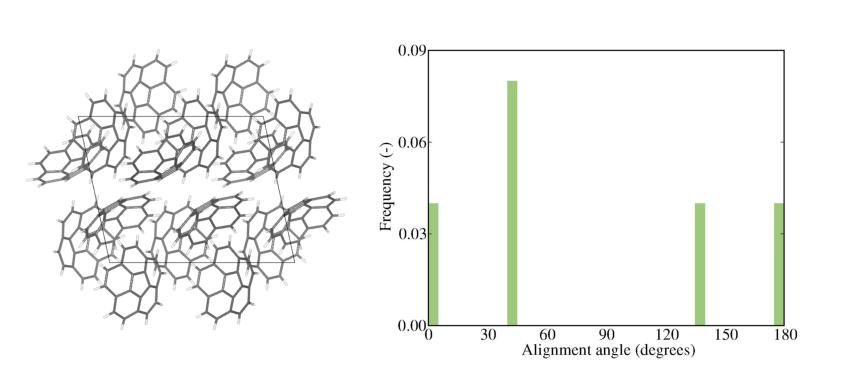
\includegraphics[width=0.65\linewidth]{Figures/corannulene_crystal.eps}
\caption{Snapshot of corannulene crystal structure (left) with alignment angle distribution (right).}
\label{fig:corannulene_crystal}
\end{figure}
%

\subsection{Cut-off distance sensitivities}
The selection of the cut-off distance, $R$, influences the calculated average intermolecular distances, coordination numbers, and alignment angles.

Due to the molecular arrangements of the homogeneous corannulene clusters (that is, sandwich-type stacking is not present), these results are the most sensitive to the selection of $R$.

- Include figure of CN histograms with r=0.5 for corannulene and 2pent15ring

- Include figures of alignment angles using R=0.5, 0.6, 0.7, 0.8 for a representative system (ann\_25?)

Note that for all systems, no neighbouring molecules are found using a cut-off distance of 0.400 nm or smaller.

\newpage

%--------------------------------------------------------------------
%     bibliography
%--------------------------------------------------------------------
\clearpage \citeindexfalse
\bibliography{c4e-preprint-bibliography}    %Create bibliography
%GATHER{c4e-preprint-bibliography.bib}      %Get WinEdt data

%--------------------------------------------------------------------
%     citation index
%--------------------------------------------------------------------
%\clearpage \makeciteindex

\end{document}

